\documentclass[12pt,a4paper]{article}
\usepackage[utf8]{inputenc}
\usepackage[T1]{fontenc} 
\usepackage[english]{babel}
\usepackage{csquotes}
\usepackage[hidelinks]{hyperref}
\usepackage{authblk}  % Add the affiliation to the author's name
\usepackage{pgfplotstable}  % TSV data support
\usepackage{graphicx}  % Table rotate support
\usepackage{rotating}  % Page rotate support
\usepackage{mfirstuc}  % For First Letter Capitalization
\usepackage{booktabs}
\usepackage{makecell}  % Enhance MultiIndex rows
\usepackage[flushleft]{threeparttable}  % For table with footnotes
\usepackage[backend=biber, % style=authoryear,
natbib=true]{biblatex}  % Bibliography support
\usepackage[acronym]{glossaries}  % Abbreviations & species support

\usepackage{tabularx}  % Extended tabular data support
\usepackage{caption}  % For extra data captions
\captionsetup{justification=raggedright,singlelinecheck=false}  % Align Caption to the left
% \renewcommand{\thetable}{(Table~\arabic{table})}  % Set table reference format

\addbibresource{latexrefs.bib}
\nonfrenchspacing

% Define macros
\newcommand{\betalactam}{$\beta$-lactam}
% Rotate & weighten items in table header
\newcommand{\rB}[1]{\rotatebox{90}{\textbf{#1}}}
% Convert cell to the union
\newcommand{\mCL}[1]{\makecell[l]{#1}}
% Reference a table
\newcommand{\refTab}[1]{(Table~\ref{tab:#1})}
% Reference a figure
\newcommand{\refFig}[1]{(Figure~\ref{fig:#1})}

% Define species
% \newacronym{<label>}{<abbrv>}{<full>}
\newacronym[first={\textit{Klebsiella pneumoniae}}]{kpne}{\textit{K. pneumoniae}}{\textit{Klebsiella pneumoniae}}
% Define abbreviations
\newacronym{bla}{BLA}{\betalactam ase}
\newacronym{bsbl}{BSBL}{broad spectrum \glsdesc{bla}}
\newacronym{ibsbl}{BSBL-inhR}{\gls{bsbl} with resistance to \glsdesc{bla} inhibitors}
\newacronym{esbl}{ESBL}{extended spectrum \glsdesc{bla}}
\newacronym{mlst}{MLST}{\textit{in silico} multi-locus sequence type}
\newacronym{mdrkp}{MDRKP}{multi drug resistant \gls{kpne}}
\newacronym{wgs}{WGS}{whole genome shotgun}

% Define authors
\author[1]{Vasilyev, I. Y.} % Corresponding author, e-mail: u0412u0418u042e@gmail.com
\author[2]{Nikolaeva, I. V.}  % irinanicolaeva@mail.ru
\author[1]{Siniagina, M. N.}  % marias25@mail.ru
\author[1]{Kharchenko, A. M.}  % anastasiahm@list.ru
\author[2]{Shaikhieva, G. S.}  % studentgulya@yandex.ru
% Define affilations
\affil[1]{Institute of Fundamental Medicine and Biology, Kazan Federal University, Kazan, Russia}
\affil[2]{Kazan State Medical University, Kazan, Russia}

\title{Multidrug-resistant hypervirulent \Gls{kpne} found persisting silently in infant gut microbiota}
\date{\today}

\begin{document}
\maketitle
\glsresetall

\begin{abstract}
\begin{minipage}{\linewidth}

\paragraph{Introduction}
% \gls{kpne} is a common microorganism and a causative agent for nosocomial infections.
Since the spread of \gls{mdrkp} strains is considered as a challenge for patients with weakened immunity,
the emergence of isolates carrying determinants of hyper virulent phenotype in addition may become a serious
problem even for healthy individuals.

\paragraph{Materials and methods.}
10 isolates were collected from 8 term neonates in maternity hospital of Kazan, Russia.
All the infants and their mothers were dismissed without complains, in satisfactory condition.
The drug resistance has been defined using a microdilution technique.
\Gls{wgs} sequencing has been performed to obtain detailed information.

\paragraph{Results.}
Phenotype analysis has confirmed production of \gls{esbl} and resistance to aminoglycosides, \betalactam,
nitrofurantoin, fluoroquinolones, sulfonamides, trimethoprim and fosfomycin antibiotics and \textit{Klebsiella} phage.
The \gls{wgs} analysis has revealed genes of resistance to aminoglycosides, fluoroquinolones, macrolides,
sulfonamides, chloramphenicol, tetracycline and trimethoprim and \gls{esbl} determinants.
The pangenome analysis had split the isolates into two phylogenetic clades.
The first, more heterogeneous clade, was represented by 5 isolates with 4 different \gls{mlst}s.
The second group contained 5 isolates from infants born vaginally with the single \gls{mlst}, ST23, positive for
genes corresponding to hyper virulent phenotype: yersiniabactin, aerobactin, salmochelin, colibactin, hypermucoidy
determinants, specific alleles of K- and O-antigens.

\paragraph{Conclusion.}
The spread of hyper virulent \gls{mdrkp} strains is a severe threat especially in a maternity hospital settings.
Therefore, this study demonstrates the case of infected infant organisms being capable to lessen the severity of disease
to asymptomatic carriage.
Since \textit{Klebsiella spp.} are known inducers of specific humoral immunity, the required antibodies
seem to be obtained by newborns vertically, from their mothers, which were immunised a time ago.

\paragraph{Keywords.}
Neonate immunity, \glsfirst{kpne}, \glsdesc{wgs}, \glsdesc{mlst}
\glsresetall

\end{minipage}
\end{abstract}


\section{Introduction}\label{sec:intro}
Newborn patients could obtain microorganisms from clinical environment, personnel, other patients and parents,
e.g.\ via breast milk.
Since Enterobacteriaceae are known early human gastrointestinal tract colonisers, local and systemic diseases could take
place during the dynamic microbiome development.
Their stabilization and persistence as may have destructive consequence on the host vital functions.
Moreover, due to the high horizontal gene transport frequency between the microbiome members, persistence of even single
strain carrying pathobiotic genes after its spread may cause explicit cyto- and genotoxic effects on host cells
leading to dangerous repercussion including colorectal cancer in particular~\cite{Pope2019}.
Underweight and weakened patients of neonatal intensive care nurseries often suffer Gram-positive bacteria infections,
mostly caused by coagulase-negative Staphylococci, while the infections caused by Gram-negative bacteria are considered
as more rare and deadly after even more rapid generalization~\cite{Dorota2017}.

\gls{kpne} is the causative agent of numerous nosocomial and community acquired infections including
pneumonia, sepsis, bacteremia, meningitis, pyogenic liver abscesses, urinary tract infections and more.
The risk group historically includes patients with weakened and malfunctioning immune system, but the spread of
hypervirulent strains also endangers immunosufficient individuals~\cite{Shankar2018}.
First isolated from lungs of patient with pneumonia \textit{postmortem}, \gls{kpne} were acknowledged as a part of
normal human gastrointestinal tract microbiome since then.
The colonization can spread, persist for years and cause different pathologies from hidden carriage to
fatal acute infections even for the healthy individuals~\cite{Martin2018}.

In this study we applied \gls{wgs} sequencing to describe in detail 8 cases of asymptomatic carriage of \gls{mdrkp}
in the gastrointestinal tract of term infants, detected at similar time periods after the birth
without visible affection on their health.
The source(s) of the \gls{mdrkp} spread was not defined.


\section{Materials and methods}\label{sec:mat_met}
\subsection{Isolation of rectal \gls{mdrkp} samples from the infant patients}\label{subsec:iso}
A total of 10 \gls{kpne} isolates demonstrating multi drug resistance phenotype were collected from 10
stool samples from 8 newborn full-term patients during hospitalization in maternity hospital of Kazan, Russia.
5 infants were born with vaginal delivery, 3~--- after cesarean surgery.
No infection outbreak was recorded and no detailed microbiological analysis was performed over parents.
The infant stool samples were collected at 3~--- 4 day of life and contaminated with $10^8$~--- $10^9$ of \gls{mdrkp}
colony-forming units per gram of stool.
The meconium samples obtained from the all 8 individuals were not tested for contamination.
Yet, the meconium samples obtained from 40 infants during the previous research were conditionally sterile or
contained lactobacteria~\cite{Nikolaeva2019a}.
Two samples collected from two infants after 1 and 6 months of monitoring also contained \gls{mdrkp}.
All the 8 babies were discharged from hospital at 4~--- 5 day of life in satisfactory condition.
Blood in stool and liquid stool were reported only once for the patient \#1 to the third month of life,
and constipation was reported for the patient \#2 to the first month of life.
No other manifested and prolonged symptoms were reported across the whole monitoring time from the all individuals.

\subsection{Phenotype Characterization}\label{subsec:phe}
The antimicrobial susceptibilities of the 10 microbial isolates were determined using a broth microdilution procedure.
The following antibacterial agents were tested: aminoglycosides (amikacin, netilmicin, gentamicin),
\betalactam s (amoxicillin-clavulanic acid, ampicillin, aztreonam, ceftriaxone, imipenem, meropenem),
nitrofuran derivatives (nitrofurantoin), sulfonamides (sulfamethoxazole), 2,4-diaminopyrimidines (trimethoprim),
fluoroquinolones (ciprofloxacin), chloramphenicol, fosfomycin.
The production of \gls{esbl} and susceptibility to \textit{Klebsiella} phage and pyo bacteriophage
were also analyzed during the routine.
The results were interpreted in automated mode using VITEK 2 Compact analyzer (bioMérieux SA, France) according to
producer's guidance documents.

\subsection{Whole-genome sequencing and assembly}\label{subsec:proc_raw}
Libraries were prepared using Nextera XT DNA Library Preparation Kit.
Whole-genome DNA was sequenced using Illumina MiSeq platform (Illumina Inc., USA),
with a paired-end run of 2 by 250 bp.
Raw reads quality control was performed with FastQC v0.11~\cite{FastQC},  % quay.io/biocontainers/fastqc:0.11.8--1
% fastqc -t 32 sample.fastq.gz -o sample
trimmed by Trimmomatic v0.39~\cite{Trimmomatic}
% quay.io/biocontainers/trimmomatic:0.39--1
% trimmomatic PE -threads 32 -phred33 sample.1.fastq.gz sample.2.fastq.gz sample_trimmomatic.1.fastq.gz sample_trimmomatic_untrimmed.1.fastq.gz sample_trimmomatic.2.fastq.gz sample_trimmomatic_untrimmed.2.fastq.gz ILLUMINACLIP:adapters.fasta:2:30:10 LEADING:3 TRAILING:3 SLIDINGWINDOW:4:15 MINLEN:36
and Cutadapt v2.4~\cite{Cutadapt},
% quay.io/biocontainers/cutadapt:2.4--py37h14c3975_0
% cutadapt -a AGATCGGAAGAG -A AGATCGGAAGAG -m 50 -o sample_cutadapt.1.fastq.gz -p sample_cutadapt.2.fastq.gz sample_trimmomatic.1.fastq.gz sample_trimmomatic.2.fastq.gz
assembled using SPAdes v3.9.1~\cite{SPAdes}.
% quay.io/biocontainers/spades:3.9.1--0
% spades --careful -o sample/genome -1 sample_cutadapt.1.fastq.gz -2 sample_cutadapt.2.fastq.gz
% spades --careful -o sample/plasmid -1 sample_cutadapt.1.fastq.gz -2 sample_cutadapt.2.fastq.gz --plasmid
Assembly statistics were calculated using the reference \gls{kpne} genome with RefSeq ID NC\_016845.1.

\subsection{Further genome assembly processing}\label{subsec:proc_ass}
The per-sample chromosome and plasmid assemblies were merged, filtered and deduplicated using in-house scripts.
The resulting assemblies were submitted to NCBI.\
The assemblies were annotated locally with Prokka v1.13.7~\cite{Prokka}
% quay.io/biocontainers/prokka:1.13.7--pl526_0
% prokka --compliant --centre UoN --cpu 32 --outdir prokka/sample --force --prefix sample --locustag sample --genus Klebsiella --species pneumoniae sample.fasta
and remotely with the NCBI Prokaryotic Genome Annotation Pipeline (PGAP)~\cite{PGAP}.
The \gls{mlst} results were computed using SRST2 v0.2~\cite{SRST2}
% quay.io/biocontainers/srst2:0.2.0--py27_2
% getmlst.py --species "Klebsiella pneumoniae"
% srst2 --output sample --input_pe sample_cutadapt.1.fastq.gz sample_cutadapt.2.fastq.gz --mlst_db Klebsiella_pneumoniae.fasta --mlst_definitions kpneumoniae.txt --mlst_delimiter '_' --log --threads 32
and Kleborate~\cite{Kleborate}.
The virulence-associated genes encoding yersiniabactin, aerobactin, salmochelin, colibactin, the regulators of mucoid
phenotype, the serotype and the drug resistance determinants were combined using Kleborate with
Kaptive subroutine~\cite{Kaptive}.
% ivasilyev/kleborate_kaptive:latest
% Kleborate --all -o results.tsv -a *.fna
Pangenome analysis was performed across the sequence query containing also 365 \gls{kpne} completed genome assemblies
downloaded from the NCBI FTP server.
A phylogeny was drawn using Roary, the Pan Genome Pipeline v3.12.0~\cite{Roary}.
% sangerpathogens/roary:latest
% roary -p 32 -f roary/ -e --mafft gff/*.gff

%%% All samples were cultured onto MacConkey agar with and without cefotaxime (2 mg/L). After incubation for 18–24 h at 37 °C, each morphotype growing on MacConkey with cefotaxime (MCA + CTX) was subjected to Gram staining, catalase and oxidase tests, followed by biochemical identification with API 20E (bioMérieux, Marcy l’Etoile, France) and the Vitek® 2 System (bioMérieux, Marcy l’Etoile, France).

\section{Results and discussion}\label{sec:res_dis}
Neonatal infection is a clinical syndrome, characterized by systemic symptoms of first month of life.
However, in this study we observed the case of newborn infant gastrointestinal tract colonization by the known
pathogen, \gls{kpne}, demonstrating a multi drug resistance phenotype without manifested symptoms.

The microdilution method has confirmed isolates with resistance to aminoglycosides, \betalactam,
nitrofuran, fluoroquinolones, sulfonamides, trimethoprim and fosfomycin antibiotics and \textit{Klebsiella} phage.
All the isolates were susceptible to amikacin, chloramphenicol and pyo bacteriophage~\refTab{phenotype}.

The discovered in \gls{wgs} \textit{de novo} resistome profile has included genetic determinants of drug resistance to
aminoglycosides, fluoroquinolones, macrolides, sulfonamides, chloramphenicol, tetracycline and trimethoprim.
It also confirmed the common \gls{bla} genes spread across the all isolates as well as the occurrence of isolates
carrying certain genes of \gls{bsbl}, \gls{ibsbl} and \gls{esbl}~\refTab{genotype}.
The results of the screening for genetic determinants of resistance to colistin, fosfomycin, glycopeptide,
nitroimidazole, rifampicin and possible production of carbapenemases or \gls{esbl} with resistance to \gls{bla}
inhibitors were negative.

Biotype profiling has revealed that 10 isolates were related to 31 reference strain and combined into two
clusters~\refFig{tree}.
The first cluster has included samples \#\# 60, 85, 91, 102 and 24.
All the isolates except the last one were obtained from the infants born with cesarean delivery.
The \gls{mlst} analysis results have included the STs 37, 45, 268 and 983\-1LV.~\refTab{genotype}
The ST37 strains were reported as possible reservoirs for carbapenem resistance genes during antimicrobial therapy
in neonates~\cite{Li2017}, the ST45~--- as the \gls{esbl}-carrying infectious agent of highly-contagious
neonatal sepsis~\cite{Marando2018}, the ST268~--- as possible reservoirs for New Delhi metallo-\gls{bla}
(NDM)~\cite{Kiaei2019}, the ST983~--- as typical causative agents of nosocomial infections
also harboring \gls{esbl}~\cite{Founou2019}.

Due to the genetic divergence within the group, the patients most likely were infected from different sources.
Since the lack of the microbiological data from detailed examination performed over their mothers, we also cannot except
the vertical transmission case, e.g.\ after the silent colonization of maternal urinary tract by \gls{mdrkp}.
It is known that asymptomatic bacteriuria occurs in 2~--- 7 \% of pregnant women in the United States
and may cause severe urinary tract infection even leading to nephrectomy~\cite{Kim2018}.
Gravidas are experiencing 20-fold increased risk of pyelonephritis mainly caused by pregnancy immunosuppression,
mechanical bladder compression and ureteral dilatation~\cite{Farkash2012}.
A vertical transmission of pathogenic microorganisms is possible during the birth and before.
The described cases of uterine \gls{kpne} infection during pregnancy include penetration via fetal membranes and
hemato-placental barrier, resulting to chorioamnionitis~\cite{Oh2017} and acute placental infection~\cite{Sheikh2005}.
The infection source for the first group of studying infants remains unclear, due to the fact that their mothers
were reported as healthy, with no symptoms or complains.

The other five isolates, \#\# 22, 90, 27, 28, 29, obtained from the infants born vaginally, have formed even less
divergent clade~\refFig{tree}, allowing us to make a conclusion about a single \gls{mdrkp} infection source.
All the 5 isolates were also positive for the genes of siderophores yersiniabactin (\textit{ybt}),
aerobactin (\textit{iuc}) and salmochelin (\textit{iro}), genotoxin colibactin (\textit{clb}),
hypermucoidy determinants (\textit{rmpA}, \textit{rmpA2}), specific \textit{wzi} loci alleles related to the
K- (capsule) and O- (LPS) antigens development which cumulative presence corresponds to extremely virulent phenotype
in theory.
More important, their \gls{mlst} was only ST23.
First reported in the mid-1980s in Taiwan, ST23 was often mentioned to present and strongly associated with the
K1 capsular serotype~\cite{Shon2013}.
The \gls{kpne} ST23 strains were confirmed as multidrug-resistant hypervirulent pathogens
caused abscesses of kidneys, pancreas, liver~\cite{Shen2019}, endogenous endophthalmitis~\cite{Xu2018},
with a dominance in the Asian-Pacific region~\cite{Thiry2019}.
In fact, it means the 4 cases of asymptomatic colonization of infant intestinal tract by hypervirulent strains of
\gls{mdrkp} which were spread a short time ago and may be accounted as a hospital-acquired infection.
The persistence of the \gls{mdrkp} ST23 strain has been also confirmed for the patient \#1 (sample \#90)
at 3rd month of life~\refTab{phenotype}~--- still without acute immune response.

The fetal immune system is not developed compared with later life mostly due to the environmental limitation~---
the stress of the own remodelling tissues and the non-inherited maternal alloantigens should not provoke
the immune reaction from the fetus side~\cite{Simon2015}.
Their innate immune system is muted~\cite{Haase2010}, the humoral immune responses are blunted,
the immunoglobulin class switching is incomplete, the released IgG antibodies decline rapidly after
immunization~\cite{Pihlgren2006}.
However, the immature Th1-type T-cell response is compensated by the IFN-$\gamma$ producing
$\gamma\delta$-T-cells~\cite{Gibbons2009}.
By the way, the main mechanism of neonatal immune protection is based on vertical transport of antibodies
via breastfeeding.
With some fortune, breastfed newborns will not suffer infections that have induced the immune response
from their mothers earlier.
Otherwise, a lack of specific antibodies will result an infection development~\cite{Dias2017}.


\section{Data availability}\label{sec:data}
The corresponding \gls{wgs} project has been deposited at NCBI GenBank database under the main
BioProject accession ID PRJNA556398.
The project data analysis scripts and materials are hosted on GitHub
(\url{https://github.com/ivasilyev/curated_projects/tree/master/inicolaeva/klebsiella_infants}).


\section{Acknowledgments}\label{sec:acks}
TODO


\printbibliography

\pagebreak
\begin{table}
\begin{threeparttable}

\caption{Patient data, sample data and demonstrated drug resistance of the studying \gls{kpne} isolates}
\label{tab:phenotype}
\centering
\noindent
\begin{tabularx}{\textwidth}{lllllllllll}
\toprule
                       Sample name & \rB{Kleb102} & \rB{Kleb22} & \rB{Kleb24} & \rB{Kleb27} & \rB{Kleb28} & \rB{Kleb29} & \rB{Kleb60} & \rB{Kleb85} & \rB{Kleb90} & \rB{Kleb91} \\
\midrule
                      Sample number &         102 &          22 &          24 &          27 &     28 &     29 &     60 &     85 &     90 &     91 \\
                           Delivery &           C &           V &           V &           V &      V &      V &      C &      C &      V &      C \\
                         Patient ID &           2 &           1 &           3 &           4 &      5 &      6 &      7 &      8 &      1 &      2 \\
                  Patient age, days &          33 &           3 &           3 &           3 &      4 &      3 &      4 &      4 &     90 &      3 \\
  \mCL{\gls{kpne},\\$\lg{CFU / g}$} &           7 &           9 &           8 &           8 &      9 &      8 &      9 &      9 &      8 &      8 \\
                         \gls{esbl} &           - &           + &           - &           - &      + &      + &      + &      + &      - &      + \\
\midrule
          \textit{Klebsiella} phage &           R &           S &           R &           R &      N &      R &      S &      S &      R &      R \\
                          Pyo phage &           S &           S &           S &           S &      S &      S &      S &      S &      S &      S \\
                           Amikacin &           S &           S &           S &           S &      S &      S &      S &      S &      S &      S \\
\mCL{Amoxicillin-\\clavulanic acid} &           R &           R &           S &           S &      R &      R &      R &      R &      S &      R \\
                         Ampicillin &           R &           R &           R &           R &      R &      R &      R &      R &      R &      R \\
                          Aztreonam &           R &           R &           S &           S &      R &      R &      R &      R &      N &      R \\
                        Ceftriaxone &           R &           R &           S &           S &      R &      R &      R &      R &      S &      R \\
                    Chloramphenicol &           N &           S &           S &           S &      S &      S &      S &      S &      S &      S \\
                      Ciprofloxacin &           S &           I &           S &           S &      R &      I &      S &      S &      S &      S \\
                         Fosfomycin &           R &           R &           I &           R &      R &      R &      R &      R &      N &      R \\
                         Gentamicin &           S &           S &           S &           N &      R &      R &      S &      S &      N &      S \\
                           Imipenem &           R &           S &           S &           I &      R &      I &      R &      R &      N &      R \\
                          Meropenem &           R &           S &           S &           S &      S &      S &      S &      S &      N &      S \\
                         Netilmicin &           S &           R &           S &           S &      R &      R &      S &      S &      N &      I \\
                     Nitrofurantoin &           R &           I &           S &           R &      R &      I &      R &      R &      R &      R \\
                   Sulfamethoxazole &           S &           R &           S &           S &      R &      R &      R &      R &      N &      R \\
                       Trimethoprim &           S &           R &           S &           S &      R &      R &      R &      R &      N &      R \\
\bottomrule
\end{tabularx}

\begin{tablenotes}
\item
Delivery: V~--- vaginal, C~--- cesarean section.
Susceptibility to the antimicrobial agent: S~-- susceptible, R~-- resistant, I~-- intermediate, N~-- not defined.
\end{tablenotes}
\end{threeparttable}
\end{table}


\pagebreak
\begin{sidewaystable}[ht]
\begin{threeparttable}
\tiny

\caption{Genome assembly data, \Acrshort{mlst}s and drug resistance determinants of the \gls{kpne} isolates}
\label{tab:genotype}
\centering
\noindent
\setlength\tabcolsep{1.5pt}  % Default value: 6pt l@{\hspace{1.5\tabcolsep}
\begin{tabularx}{\textwidth}{lllllllllll}
\toprule
                   Sample name &       \textbf{Kleb102} &                  \textbf{Kleb22} &   \textbf{Kleb24} &          \textbf{Kleb27} &                 \textbf{Kleb28} &                \textbf{Kleb29} &                  \textbf{Kleb60} &         \textbf{Kleb85} &                  \textbf{Kleb90} &         \textbf{Kleb91} \\
\midrule
                  Accession ID &           VOOJ00000000 &                     VOOA00000000 &      VOOC00000000 &             VOOD00000000 &                    VOOE00000000 &                   VOOF00000000 &                     VOOG00000000 &            VOOH00000000 &                     VOOB00000000 &            VOOI00000000 \\
                  Reads number &                1040088 &                           805318 &            856300 &                  1056762 &                          926382 &                        1259976 &                           994296 &                 1207354 &                          1216382 &                 1381726 \\
                      Coverage &                  58.7x &                            45.4x &             48.3x &                    59.6x &                           52.3x &                          71.1x &                            56.1x &                   68.1x &                            68.6x &                   78.0x \\
\mCL{Genome\\assembly\\length} &                5297684 &                          5881113 &           5518356 &                  5641111 &                         5885411 &                        5890967 &                          5666743 &                 5324705 &                          5882697 &                 5326604 \\
                Contigs number &                    106 &                              111 &                94 &                       76 &                             120 &                            118 &                               91 &                      74 &                              108 &                      77 \\
                    N50 metric &                 350001 &                           307112 &            319410 &                   322041 &                          307112 &                         307112 &                           263911 &                  358425 &                           307112 &                  437151 \\
 \mCL{Largest\\contig\\length} &                1106296 &                           770102 &            930837 &                  1334922 &                          771547 &                         799268 &                           642551 &                  812552 &                           799226 &                  812552 \\
\midrule
                    \gls{mlst} &              ST983-1LV &                             ST23 &              ST37 &                     ST23 &                            ST23 &                           ST23 &                            ST268 &                    ST45 &                             ST23 &                    ST45 \\
                Yersiniabactin &                   ybt? &            \mCL{ybt 1,\\ICEKp10} &                 - &    \mCL{ybt 1,\\ICEKp10} &           \mCL{ybt 1,\\ICEKp10} &          \mCL{ybt 1,\\ICEKp10} &           \mCL{ybt 17,\\ICEKp10} &                       - &            \mCL{ybt 1,\\ICEKp10} &                       - \\
                    Colibactin &                      - &                            clb 2 &                 - &                    clb 2 &                           clb 2 &                          clb 2 &                            clb 3 &                       - &                            clb 2 &                       - \\
                    Aerobactin &                      - &                            iuc 1 &                 - &                    iuc 1 &                           iuc 1 &                          iuc 1 &                            iuc 1 &                       - &                            iuc 1 &                       - \\
                   Salmochelin &                      - &                            iro 1 &                 - &                    iro 1 &                           iro 1 &                          iro 1 &                            iro 1 &                       - &                            iro 1 &                       - \\
                 \textit{rmpA} &                      - &         \mCL{rmpA$_2$\\(KpVP-1)} &                 - & \mCL{rmpA$_2$\\(KpVP-1)} &        \mCL{rmpA$_2$\\(KpVP-1)} &       \mCL{rmpA$_2$\\(KpVP-1)} &        \mCL{rmpA$_2$*\\(KpVP-1)} &                       - &         \mCL{rmpA$_2$\\(KpVP-1)} &                       - \\
                \textit{rmpA2} &                      - &                        rmpA2$_8$ &                 - &                rmpA2$_5$ &                       rmpA2$_8$ &                      rmpA2$_8$ &                       rmpA2$_2$* &                       - &                        rmpA2$_8$ &                       - \\
                  \textit{wzi} &                  wzi39 &                             wzi1 &            wzi123 &                     wzi1 &                            wzi1 &                           wzi1 &                            wzi95 &                  wzi101 &                             wzi1 &                  wzi101 \\
                       K locus &                   KL39 &                              KL1 &             KL136 &                      KL1 &                             KL1 &                            KL1 &                             KL20 &                    KL24 &                              KL1 &                    KL24 \\
                       O locus &                    O3b &                             O1v2 &              O2v2 &                     O1v2 &                            O1v2 &                           O1v2 &                             O2v1 &                    O2v1 &                             O1v2 &                    O2v1 \\
               Aminoglycosides &     \mCL{StrB,\\StrA*} &   \mCL{StrB,\\StrA*,\\Aac3-IIa*} & \mCL{StrB,\\StrA} &                        - &  \mCL{StrB,\\StrA*,\\Aac3-IIa*} & \mCL{StrB,\\StrA*,\\Aac3-IIa*} &    \mCL{StrB,\\StrA*,\\Aph3-Ia*} &      \mCL{StrB,\\StrA*} &   \mCL{StrB,\\StrA*,\\Aac3-IIa*} &      \mCL{StrB,\\StrA*} \\
              Fluoroquinolones &                      - &                           QnrB1? &                 - &                        - &                          QnrB1? &                         QnrB1? &                                - &                       - &                           QnrB1? &                       - \\
                    Macrolides &                      - &                                - &                 - &                        - &                               - &                              - &                            EreA2 &                       - &                                - &                       - \\
                     Phenicols &                 CatA1* &                            CatB4 &                 - &                        - &                           CatB4 &                          CatB4 &                                - &                   CatB4 &                            CatB4 &                   CatB4 \\
                  Sulfonamides &                 SulII* &              \mCL{SulII,\\SulII} &                 - &                        - &                           SulII &                          SulII &              \mCL{SulI,\\SulII*} &                   SulII &                            SulII &                   SulII \\
                 Tetracyclines &                   TetA &                             TetA &                 - &                        - &                            TetA &                           TetA &                                - &                       - &                             TetA &                       - \\
                  Trimethoprim &                      - &                           DfrA14 &                 - &                        - &                          DfrA14 &                         DfrA14 &                            DfrA5 &                  DfrA14 &                           DfrA14 &                  DfrA14 \\
                     \gls{bla} & \mCL{SHV-187*,\\AmpH*} &    \mCL{SHV-190*,\\AmpH,\\OXA-1} &             AmpH* &    \mCL{SHV-190*,\\AmpH} &   \mCL{SHV-190*,\\AmpH,\\OXA-1} &  \mCL{SHV-190*,\\AmpH,\\OXA-1} &                            AmpH* &     \mCL{AmpH*,\\OXA-1} &    \mCL{SHV-190*,\\AmpH,\\OXA-1} &     \mCL{AmpH*,\\OXA-1} \\
                    \gls{esbl} &                      - &                         CTX-M-15 &                 - &                        - &                        CTX-M-15 &                       CTX-M-15 &           \mCL{SHV-13*, CTX-M-3} &                CTX-M-15 &                         CTX-M-15 &                CTX-M-15 \\
                    \gls{bsbl} &                      - &                                - &           SHV-77* &                        - &                               - &                              - &                                - &                       - &                                - &                       - \\
                   \gls{ibsbl} &                TEM-30* &                          TEM-30* &                 - &                        - &                         TEM-30* &                        TEM-30* &                                - & \mCL{SHV-26*,\\TEM-30*} &          \mCL{TEM-30*,\\TEM-30*} & \mCL{SHV-26*,\\TEM-30*} \\
\bottomrule
\end{tabularx}

\begin{tablenotes}
\item
\gls{mlst}~--- \glsdesc{mlst}, \gls{bla}~--- \glsdesc{bla}, \gls{bsbl}~--- \glsdesc{bsbl},
\gls{ibsbl}~--- \glsdesc{ibsbl}, \gls{esbl}~--- \glsdesc{esbl}.
\end{tablenotes}
\end{threeparttable}
\end{sidewaystable}


\pagebreak
\begin{figure}[h]
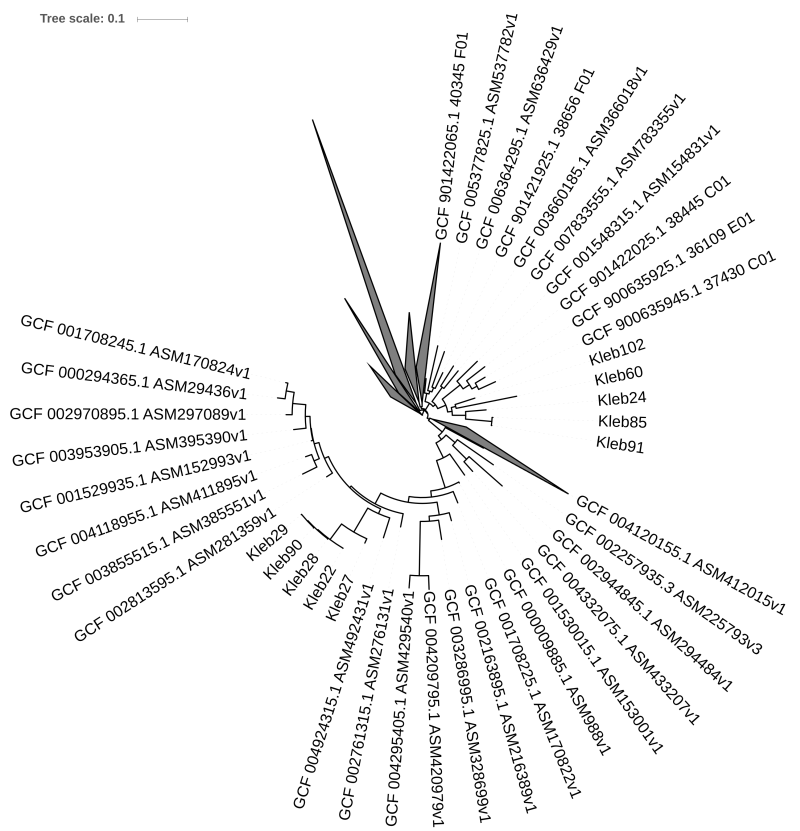
\includegraphics[width=0.9\textwidth]{png/tree.png}
\caption{Corresponding dendrogram determined with Roary pangenome pipeline in reference and studying
isolates of \gls{kpne}}
\label{fig:tree}
\end{figure}

\pagebreak
% Compiled from \LaTeXe{}.
% \pagebreak
\end{document}
